% Compile with XeLaTeX (required for the Bangla examples).
%   xelatex acl_latex && bibtex acl_latex && xelatex acl_latex && xelatex acl_latex
\documentclass[11pt]{article}

% Change "review" to "final" to generate the final (sometimes called camera-ready) version.
% Change to "preprint" to generate a non-anonymous version with page numbers.
\usepackage[review]{acl}

\usepackage{microtype}
\usepackage{graphicx}
\usepackage{booktabs}
\usepackage{amsmath}
\usepackage{xcolor}

% These font commands require XeLaTeX or LuaLaTeX, not pdfLaTeX.
\usepackage{fontspec}
\setmainfont{TeX Gyre Termes}          % Times-compatible, per the ACL template
\newfontfamily\bnfont[Path=./,Script=Bengali,Renderer=HarfBuzz]{kalpurush.ttf}

% Bangla inline span. Script=Bengali enables the GSUB conjunct substitutions,
% without which ligatures such as ভান্তে and ব্রাহ্মণ render as broken glyph
% sequences.
\newcommand{\bn}[1]{{\bnfont #1}}
% Bangla term followed by transliteration and gloss.
\newcommand{\bng}[3]{\bn{#1} \textit{#2} `#3'}

% Details that only the authors can supply; see SUBMISSION_CHECKLIST.md.
\newcommand{\authorfill}[1]{\textcolor{red}{[#1]}}

\title{Model, Not Culture: What Expert Ratings of 599 LLM-Generated Bangla
Folk Stories Do and Do Not Measure}

\author{Anonymous ACL submission}

\begin{document}
\maketitle

\begin{abstract}
We present JAF, a corpus of 599 Bangla folk stories generated by five large
language models for twelve Bangladeshi cultures across ten narrative types,
each rated by four expert annotators on four dimensions
(9{,}584 judgments, Krippendorff's $\alpha = 0.81$--$0.87$).
Every model falls below the scale midpoint on every dimension, and the best
model reaches only 2.79 of 5. Pairing the ratings with a quantitative analysis
of the generated text itself yields three findings that neither source gives
alone. First, which model wrote a story explains $24\times$ more rating
variance than which culture it depicts ($R^2 = 0.395$ vs.\ $0.017$): the
benchmark separates model capability, not differential cultural difficulty.
Second, lexical culture-marking dissociates from judged authenticity. A
classifier recovers the target culture from text at $0.466$ accuracy with
ethnonyms masked, but the most separable model is rated fourth of five, and the
weakest model falls \emph{below} the $1/12$ chance baseline. Automatic
culture-separability would invert the expert ranking. Third, the failure is omission rather than
rationalisation: across the 100 stories for the two Christian-majority
communities not one contains a Christian marker, while the scientific register
that folk-tale rationalisation would predict appears in 2.7\% of stories and is
flat across narrative types. We release the corpus, the annotations, and the
analysis code.
\end{abstract}

\section{Introduction}

Folk narrative is a demanding test of what a language model knows about a
culture. A folk tale is not a list of facts to be recalled but a performance
that must sustain a register, a cosmology, a social world and a moral logic
simultaneously, and a reader from inside the tradition notices when any of
these slips. This makes generation a sharper probe than the
multiple-choice formats that dominate cultural evaluation
\cite{Myung2024,chiu-etal-2025-culturalbench,Etxaniz2024}, which can only ask
whether a fact is retrievable.

Bangladesh offers an unusually well-controlled setting for such a probe. Beside
the Bengali majority live dozens of distinct communities --- Chakma, Marma,
Mro, Khasi, Garo, Santal, Oraon and others --- that share a national context
and, increasingly, a written language, while differing sharply in religion,
kinship, subsistence and ritual. Holding the output language fixed at standard
Bangla and varying only the target community isolates cultural competence from
multilingual competence. Existing Bangla NLP resources evaluate summarisation,
style transfer and general capability
\cite{bhattacharjee-etal-2023-banglanlg,khan-etal-2023-banglachq,kabir-etal-2024-benllm,mukherjee-etal-2023-low},
and recent work probes Bengali cultural \emph{knowledge}
\cite{chowdhury-etal-2025-facts}, but the generative question for Bangladesh's
minority communities is largely untouched; of the twelve communities we study,
only Chakma \cite{rahman-etal-2025-chakmabridge} and Khasi
\cite{ghosh-etal-2025-towards} appear in the NLP literature at all.

We introduce \textbf{JAF}, a fully crossed corpus: 12 cultures $\times$ 10
story types $\times$ 5 models, every story rated by the same four experts on
cultural accuracy, contextual and temporal appropriateness, narrative and
symbolic coherence, and linguistic and expressive appropriateness. The design
makes culture a controlled variable rather than a case study, which turns out
to matter: the closest prior work \cite{pranida-etal-2025-culturally} reports
that LLM-generated stories match native-written ones on cultural fidelity for
Javanese and Sundanese, and that conclusion does not survive widening the
culture axis from two to twelve.

Our contribution is not only the ratings. We pair them with a quantitative
analysis of the 599 texts --- stylometry, classifier-based identifiability,
curated religious and register lexicons --- and the combination answers
questions that neither source answers alone. Concretely:

\begin{itemize}\itemsep1pt
\item \textbf{Model dominates culture.} Model identity explains $R^2 = 0.395$
of mean-rating variance; culture explains $0.017$ and story type $0.003$
(\S\ref{sec:variance}).
\item \textbf{Separability is not authenticity.} Culture identifiability and
expert rating dissociate completely across models, so any automatic
culture-separability metric would rank the models wrongly
(\S\ref{sec:flattening}). This is the empirical case for expert evaluation.
\item \textbf{The failure is omission, not rationalisation.} Expected
religious register is absent --- entirely so for two communities --- while the
scientific-intrusion hypothesis is falsified (\S\ref{sec:register}).
\item \textbf{Surface features predict nothing within a model.} Length
correlates with rating at $\rho = 0.36$ pooled and $\approx 0$ inside every
model --- a warning for anyone building automatic proxies on corpora like this
(\S\ref{sec:confound}).
\end{itemize}

\section{Related Work}

\paragraph{Cultural benchmarks for LLMs.}
A growing family of benchmarks measures cultural knowledge through
classification or multiple choice: BLEnD on everyday knowledge across cultures
\cite{Myung2024}, CulturalBench \cite{chiu-etal-2025-culturalbench}, BertaQA on
local Basque knowledge \cite{Etxaniz2024}, IndoCulture on geographically
grounded Indonesian commonsense \cite{koto-etal-2024-indoculture}, NormAd on
cultural adaptability \cite{rao-etal-2025-normad}, and WorldValuesBench on
value prediction \cite{zhao-etal-2024-worldvaluesbench}. CultureBank
\cite{shi-etal-2024-culturebank} builds a community-sourced knowledge base, and
CulFiT \cite{feng-etal-2025-culfit} uses cultural critique for training.
\citet{alkhamissi-etal-2024-investigating} study cultural alignment directly,
and \citet{chae-etal-2025-assessing} question whether sovereign LLMs serve
their target populations as claimed. These share a format constraint: they ask
whether a model can \emph{select} a culturally correct answer, not whether it
can \emph{sustain} a culturally coherent text.

\paragraph{Folklore and narrative generation.}
\citet{wu-etal-2023-cross} analyse values and gender bias across 1{,}900
human-written tales from 27 cultures, establishing folk narrative as a
tractable object of computational study but not evaluating generation.
\citet{tsutsumi-jinnai-2025-large} probe folktale knowledge with YokaiEval, 809
multiple-choice questions on Japanese \textit{yokai}, and find that
Japanese-resourced models outperform English-centric ones --- again a knowledge
format. \citet{razumovskaia-etal-2024-little} study crosslingual story
planning, \citet{yunusov-etal-2024-mirrorstories} personalised narrative, and
\citet{mitran-etal-2025-probing} moral foundations in generated narrative.
\citet{bhandari-brennan-2023-trustworthiness} evaluate the trustworthiness of
LLM-generated children's stories, and \citet{delucia-etal-2021-decoding}
examine decoding for narrative generation.

The closest work is \citet{pranida-etal-2025-culturally}, which generates
culturally nuanced stories for Javanese and Sundanese and reports that LLM
stories match native-written ones on cultural fidelity while lagging on
coherence. Our design differs in three ways that matter for that claim: twelve
cultures rather than two, four experts rating every item rather than a sample,
and a majority-language control condition (Bengali) inside the same corpus.
Under those conditions the fidelity parity does not reproduce
(\S\ref{sec:flattening}).

\paragraph{Bangla and low-resource NLP.}
Bangla has benchmarks for generation and summarisation
\cite{bhattacharjee-etal-2023-banglanlg,khan-etal-2023-banglachq}, LLM
evaluation \cite{kabir-etal-2024-benllm}, style transfer
\cite{mukherjee-etal-2023-low} and poetic form \cite{amina-etal-2025-form}.
\citet{chowdhury-etal-2025-facts} introduce BLanCK for Bengali cultural
knowledge including folk traditions and find that supplying context
substantially improves performance --- evidence that the gap is partly
retrieval rather than absence, which motivates our proposed ablation
(\S\ref{sec:discussion}). For Bangladesh's minority communities the resource
situation is far thinner: ChakmaBridge \cite{rahman-etal-2025-chakmabridge}
provides a parallel corpus for Chakma, and \citet{ghosh-etal-2025-towards}
develop annotated resources for Mizo and Khasi. Work on other low-resource
settings \cite{azime-etal-2024-walia,meaney-etal-2024-testing,razumovskaia-etal-2024-little}
and on evaluation trustworthiness \cite{bhandari-brennan-2023-trustworthiness}
informs our protocol. To our knowledge no prior work evaluates
\emph{generation} for these communities, with \emph{expert} multi-dimensional
rating, treating \emph{culture as a controlled variable}.

\section{The JAF Corpus}
\label{sec:corpus}

\paragraph{Design.}
The corpus crosses 12 cultures, 10 story types and 5 models. Cultures are
Bengali, Chakma, Marma, Santal, Garo (Mandi), Khasi, Manipuri (Meitei), Mro,
Tripura, Hajong, Rakhine and Oraon (Kurukh). They span four unrelated
language families, three cultural-geographic zones and five religious
traditions, and range from 483{,}299 people (Chakma) to 7{,}996 (Hajong) in
the 2022 census \cite{bbs2022census}. Appendix~\ref{sec:cultures} describes
each community and documents the sources behind the expected-tradition
mapping used in \S\ref{sec:register}. Story types are Origin Story,
Human--Nature Relationship, Moral Transgression and Consequence, Wisdom of an
Elder, Community Crisis, Rite of Passage, Trickster or Clever Figure, Sacred or
Forbidden Space, Everyday Life Narrative, and Change and Continuity. Each
(culture, type) pair is one prompt, giving 120 prompts; each prompt is sent to
all five models. One cell (P091, Origin Story, North Bengal, qwen3-8b) is
missing, giving 599 stories rather than 600.

\paragraph{Prompt.}
A single Bangla prompt template is used throughout, instantiated with the
culture name and the story-type scenario. It casts the model as a folk
storyteller (\bn{লোককথা-কথক} \textit{lokkatha-kothok}), requires standard Bangla while permitting
regionally appropriate vocabulary, and imposes three explicit constraints:
write approximately 500--700 words; do not use modern technology, modern
statecraft, specific years or contemporary vocabulary; and do not invent
specific details the model is unsure of. These constraints are directly
measurable, and we report compliance in \S\ref{sec:register}.

\paragraph{Models.}
We evaluate \texttt{openai\_gpt-5.1}, \texttt{openai\_gpt-5-mini},
\texttt{google\_gemini-3-flash-preview},
\texttt{mistralai\_mistral-large-2512} and \texttt{qwen\_qwen3-8b}, spanning
frontier, efficient and small open-weight tiers.
\authorfill{AUTHORS: add decoding parameters (temperature, top-p, max tokens),
access route and dates, and the exact provider snapshot for each model.}

\paragraph{Annotation.}
Four expert annotators rated every one of the 599 stories on a 0--5 scale along
four dimensions: cultural accuracy and authenticity, contextual and temporal
appropriateness, narrative and symbolic coherence, and linguistic and
expressive appropriateness. This yields 9{,}584 judgments with no missing
cells.
\authorfill{AUTHORS: required for the Responsible NLP checklist (D1--D5) --- the full
rubric with level descriptors, annotator recruitment, cultural and linguistic
background of each annotator relative to the twelve communities, compensation,
consent, training/calibration procedure, and IRB status or exemption. We cannot
infer these from the released artifact.}

\paragraph{Agreement.}
Table~\ref{tab:agreement} reports Krippendorff's $\alpha$ with the ordinal
difference metric and ICC(2,k). Agreement is substantial on all four
dimensions. Linguistic register is both the lowest-agreement and the
lowest-scoring dimension: experts agree least about precisely what models do
worst.

\begin{table}[t]
\centering\small
\begin{tabular}{lccc}
\toprule
Dimension & $\alpha$ & ICC(2,k) & exact \\
\midrule
Cultural accuracy    & 0.862 & 0.956 & 74.1\% \\
Contextual fit       & 0.871 & 0.960 & 75.1\% \\
Narrative coherence  & 0.848 & 0.946 & 77.0\% \\
Linguistic register  & 0.805 & 0.941 & 68.1\% \\
\bottomrule
\end{tabular}
\caption{Inter-annotator agreement over 4 experts $\times$ 599 items.
``exact'' is the share of items where all four experts gave the identical
score.}
\label{tab:agreement}
\end{table}

\section{Expert Ratings}
\label{sec:ratings}

\begin{table}[t]
\centering\small
\setlength{\tabcolsep}{3.5pt}
\begin{tabular}{lccccc}
\toprule
Model & Cult. & Ctx. & Narr. & Ling. & All \\
\midrule
gpt-5.1        & \textbf{3.11} & \textbf{3.02} & \textbf{2.73} & \textbf{2.31} & \textbf{2.79} \\
gpt-5-mini     & 2.39 & 2.03 & 1.93 & 1.55 & 1.97 \\
gemini-3-flash & 2.44 & 1.96 & 1.91 & 1.45 & 1.94 \\
qwen3-8b       & 2.14 & 2.09 & 1.83 & 1.33 & 1.85 \\
mistral-large  & 2.23 & 1.85 & 1.74 & 1.19 & 1.75 \\
\bottomrule
\end{tabular}
\caption{Mean expert ratings (0--5). Every cell is below the 2.5 midpoint
except gpt-5.1 on cultural accuracy and contextual fit.}
\label{tab:models}
\end{table}

\begin{figure}[t]
\centering
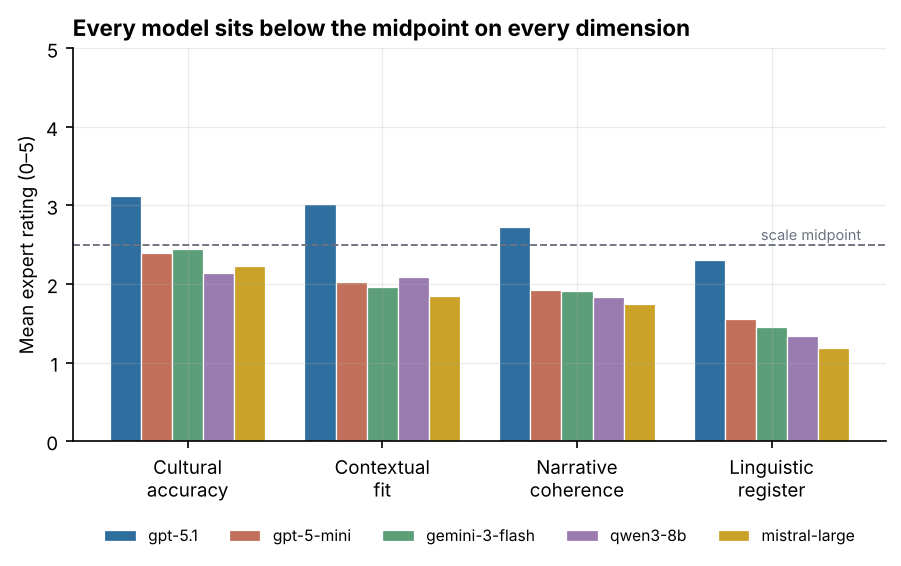
\includegraphics[width=\columnwidth]{figures/fig1_model_by_dimension.png}
\caption{Mean expert rating by model and dimension. Linguistic register is the
floor for every model.}
\label{fig:models}
\end{figure}

Table~\ref{tab:models} and Figure~\ref{fig:models} give the headline result.
The ceiling is 2.79 of 5.
Four of five models sit below the scale midpoint on every dimension, and the
ordering is stable across dimensions. This is not a leaderboard in which a
winner has solved the task; it is a uniform failure with one model failing
less.

Two patterns recur. First, \textbf{linguistic register is the floor for every
model}, ranging 1.19--2.31 and always the worst of the four dimensions. Models
retrieve cultural content more successfully than they sustain the register a
folk tale requires. The four dimensions correlate only at $r = 0.41$--$0.45$,
so they are not collapsing into a single latent quality factor. Second,
\textbf{culture barely matters}: the twelve communities span 2.21 (Hajong) to
1.95 (Chakma), a range narrower than the gap between any two adjacent models.
Bengali, by far the highest-resourced of the twelve, scores 2.13 --- mid-pack,
below Hajong and Mro. The failure is not a simple function of resource
scarcity.

A third observation concerns the scale itself. Judgments concentrate in the
1--3 band: across all 9{,}584 ratings the upper half of the scale is used
sparingly, and no model has a mean above 3.11 on any dimension. The restricted
range means agreement statistics that depend on between-item variance should be
read with care, and it limits the headroom available to distinguish the four
lower-ranked models, which span only 1.75--1.97.

\subsection{Variance decomposition}
\label{sec:variance}

\begin{table}[t]
\centering\small
\begin{tabular}{lc}
\toprule
Factor & $R^2$ on mean rating \\
\midrule
\textbf{Model}        & \textbf{0.395} \\
Culture               & 0.017 \\
Region                & 0.015 \\
Story type            & 0.003 \\
\midrule
Model + culture + type & 0.414 \\
\bottomrule
\end{tabular}
\caption{One-way $R^2$ of each design factor on mean expert rating,
$n = 599$.}
\label{tab:variance}
\end{table}

Table~\ref{tab:variance} quantifies the asymmetry. Model identity explains
$24\times$ more rating variance than target culture and roughly $130\times$
more than story type; adding culture and story type to a model-only regression
buys $0.019$ of $R^2$.

This has a direct consequence for how such benchmarks should be read. A corpus
of this shape invites the interpretation that some cultures are harder than
others, and the data does not support it. What the ratings principally measure
is general generation capability expressed in Bangla. Cultural variation is
real but second-order, and any claim about per-culture difficulty needs far
more power than twelve cultures $\times$ five models provides.

\section{Beyond the Ratings}
\label{sec:beyond}

We now analyse the 599 texts themselves. All measures operate on Bangla-script
word tokens with a light inflectional suffix matcher, not raw substrings; this
is not a detail. A naive substring search reports \bn{গ্রহ} \textit{graha} (`planet') in
105 stories, of which essentially all are the unrelated \bn{গ্রহণ} \textit{grahan}
(`to accept'), and \bn{বাস} \textit{bas} (`bus') appears to occur in 503 stories because it is
a substring of \bn{বসবাস} \textit{basbas} (`to dwell'). Substring counting would have
produced a spurious modernity signal an order of magnitude too large.

\subsection{Models are perfectly separable}
\label{sec:stylometry}

A TF-IDF and logistic-regression classifier recovers which model generated a
story with \textbf{100.0\%} five-fold cross-validated accuracy (chance 20\%).
Table~\ref{tab:stylometry} shows why: the stylistic signatures are
categorical, not statistical. Mistral emits a bolded Markdown title on
\emph{every} story and qwen on 97.5\%, while the OpenAI models essentially
never do --- a formatting artifact in a corpus of purportedly oral narrative.
79\% of qwen stories contain a repeated 4-gram.

\begin{table}[t]
\centering\small
\setlength{\tabcolsep}{3pt}
\begin{tabular}{lccccc}
\toprule
 & gem. & mis. & mini & 5.1 & qwen \\
\midrule
Mean tokens      & 593 & 478 & 596 & 987 & 332 \\
MATTR-50         & .91 & .87 & .92 & .92 & .80 \\
Markdown bold    & 1\% & 100\% & 0\% & 3\% & 98\% \\
Em-dash /1k      & 4.0 & 10.4 & 35.5 & 19.6 & 1.3 \\
Oral framing     & .84 & .38 & .46 & .69 & .04 \\
Moral coda       & 27\% & 28\% & 21\% & 8\% & 14\% \\
Rep.\ 4-gram     & .000 & .007 & .000 & .001 & .042 \\
\bottomrule
\end{tabular}
\caption{Stylometric signatures. Oral framing counts distinct
audience-addressing devices; moral coda is an explicit ``the lesson is''
closing.}
\label{tab:stylometry}
\end{table}

\subsection{Cultural flattening, measured}
\label{sec:flattening}

If models genuinely differentiate twelve cultures, a classifier should separate
them. On raw text, 12-way cross-validated accuracy is $0.601$. After masking
ethnonyms and giveaway place names, it falls to $\mathbf{0.466}$: roughly a
quarter of the apparent cultural signal was the model naming the group.

Per model, after masking (chance $= 0.083$):

\begin{table}[h]
\centering\small
\begin{tabular}{lcc}
\toprule
Model & Culture acc. & Rating \\
\midrule
gemini-3-flash & \textbf{0.708} & 1.94 \\
gpt-5.1        & 0.617 & \textbf{2.79} \\
mistral-large  & 0.383 & 1.75 \\
gpt-5-mini     & 0.225 & 1.97 \\
qwen3-8b       & \textbf{0.067} & 1.85 \\
\bottomrule
\end{tabular}
\caption{Culture identifiability (ethnonyms masked) against mean expert
rating. qwen3-8b falls below the $1/12$ chance baseline.}
\label{tab:ident}
\end{table}

Two results follow. First, \textbf{qwen3-8b falls below chance}: its 119
stories carry essentially no information about which of twelve communities they
depict. It writes one story --- typically opening ``in a small village in
Bangladesh'' --- and changes the label.

Second, and more consequential for evaluation methodology,
\textbf{differentiation and authenticity dissociate}
(Figure~\ref{fig:ident}). Gemini is the most culturally separable model and is
rated fourth of five; gpt-5.1 is less separable and rated first. Gemini varies
its vocabulary across cultures reliably while reaching for markers that experts
judge wrong: it is internally consistent and externally incorrect, a
combination a classifier rewards and a cultural expert penalises. An automatic
culture-separability metric --- the kind that is attractive precisely because
expert annotation is expensive --- would invert the expert ranking on this
corpus. We take this as the central methodological argument for
expert evaluation in culturally grounded generation.

\begin{figure}[t]
\centering
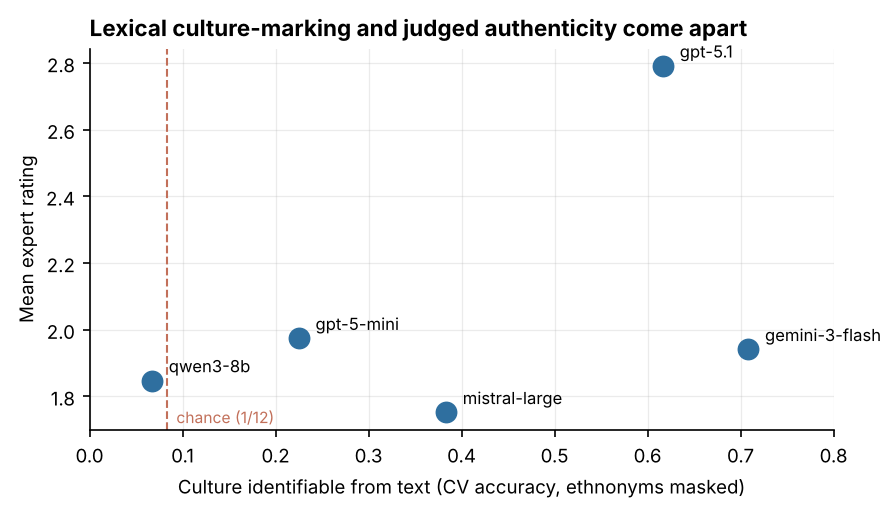
\includegraphics[width=\columnwidth]{figures/fig3_identifiability_vs_rating.png}
\caption{Culture identifiability (ethnonyms masked) against mean expert rating.
The two measures are unrelated across models.}
\label{fig:ident}
\end{figure}

Confusions are geographically coherent rather than arbitrary:
Chakma$\leftrightarrow$Tripura (19 errors), Mro$\leftrightarrow$Tripura (16),
Oraon$\leftrightarrow$Santal (12) and Chakma$\leftrightarrow$Marma (12) are all
Chittagong-Hill-Tracts or northwestern-plains neighbours. Models blur real
adjacencies rather than failing randomly.

Aggregate cultural knowledge in the corpus is nonetheless real.
Table~\ref{tab:distinctive} lists the most distinctive content words per
culture by log-odds ratio with an informative Dirichlet prior, and the terms
are overwhelmingly appropriate: the Santal sacred grove and supreme deity, the
Garo village headman and harvest festival, the Oraon festival, priest and
drum, the Rakhine monastery. The knowledge exists in aggregate; it is unevenly
and often incorrectly deployed per story. The Manipuri row shows the leak
discussed below --- \bn{মণ্ডপ} \textit{mandap} and \bn{মন্দির} \textit{mandir} sit beside the
correct \bn{লাই} \textit{lai}.

\begin{table}[t]
\centering\small
\setlength{\tabcolsep}{3pt}
\begin{tabular}{@{}lp{5.4cm}@{}}
\toprule
Culture & Most distinctive content words \\
\midrule
Bengali  & \bng{কুকুর}{kukur}{dog}, \bng{পুজো}{pujo}{worship}, \bng{শিয়াল}{shiyal}{jackal}, \bng{পিঠা}{pitha}{rice cake} \\
Chakma   & \bng{ঝিরি}{jhiri}{hill stream}, \bng{জুম}{jum}{swidden}, \bng{কারবারি}{karbari}{headman}, \bng{ভান্তে}{bhante}{monk} \\
Marma    & \bng{সাঙ্গু}{Sangu}{river}, \bng{কিয়াং}{kyang}{monastery}, \bng{পাহাড়}{pahar}{hills} \\
Santal   & \bng{জাহের}{jaher}{sacred grove}, \bng{মারাং}{marang}{Marang Buru}, \bng{মাঝি}{majhi}{headman}, \bng{থান}{than}{shrine} \\
Garo     & \bng{নকমা}{nokma}{village chief}, \bng{ওয়ানগালা}{Wangala}{harvest festival}, \bng{সিমসাং}{Simsang}{river} \\
Khasi    & \bng{পান}{pan}{betel}, \bng{সুপারি}{supari}{areca}, \bng{পুঞ্জি}{punji}{hamlet} \\
Manipuri & \bng{লাই}{lai}{deity}, \bng{মণ্ডপ}{mandap}{pavilion}, \bng{মন্দির}{mandir}{temple} \\
Mro      & \bng{পাড়া}{para}{hamlet}, \bng{শূকর}{shukor}{pig}, \bng{জুম}{jum}{swidden} \\
Tripura  & \bng{খোক্কো}{khokko}{ogre}, \bng{জুম}{jum}{swidden}, \bng{হরিণ}{horin}{deer} \\
Hajong   & \bng{ধান}{dhan}{paddy}, \bng{সোমেশ্বরী}{Someshwari}{river}, \bng{ঠাকুমা}{thakuma}{grandmother} \\
Rakhine  & \bng{নৌকা}{nouka}{boat}, \bng{সমুদ্র}{samudra}{sea}, \bng{কিয়াং}{kiyang}{monastery} \\
Oraon    & \bng{করম}{karam}{festival}, \bng{পাহান}{pahan}{priest}, \bng{মাদল}{madal}{drum}, \bng{শাল}{shal}{sal tree} \\
\bottomrule
\end{tabular}
\caption{Top distinctive content words per culture (log-odds with informative
Dirichlet prior). Personal names omitted.}
\label{tab:distinctive}
\end{table}

\subsection{Expected religious register is missing}
\label{sec:register}

We score each story against the tradition that actually predominates in its
target community, using lexicons of tradition-specific markers. The mapping
from community to expected tradition follows the Banglapedia community entries
and is tabulated with sources in Appendix~\ref{sec:cultures}
\cite{banglapedia}.

The most robust result is an \emph{absence}. Across the 100 stories written for
the two Christian-majority communities --- Garo, most of whom are Christian,
and Khasi, over 80\% of whom are \cite{banglapedia-garo,banglapedia-khasia}
--- not one contains a Christian marker (\bn{গির্জা} \textit{girja} `church', \bn{যীশু}
\textit{Jishu} `Jesus', \bn{পাদ্রি} \textit{padri} `priest', and related
terms): 0.0\%. Correct-tradition markers of any kind appear in only 6\% of Garo
and 6\% of Khasi stories, against 48\% for Marma and 64\% for Manipuri
(Figure~\ref{fig:religion}). The models do not merely under-represent these
communities' religious life; for two of them they omit it entirely. Presence of
a correct-tradition marker is associated with higher cultural accuracy across
the corpus (2.578 vs.\ 2.410, Mann--Whitney $p = 0.026$, $d = +0.21$).

\paragraph{Leakage, tiered.} A natural companion claim is that Hindu register
leaks into non-Hindu communities. Taken at face value, 20.8\% of non-Bengali
stories contain a strictly Hindu marker. That figure needs qualifying, and we
report the qualification because it materially weakens the claim. Bangla has no
religiously neutral everyday vocabulary for several ritual concepts, so a model
writing about a Santal \bn{নায়কে} \textit{naeke} in Bangla may gloss the role
as \bn{পুরোহিত} \textit{purohit} `priest' and the rite as \bn{পূজা}
\textit{puja} `worship' without importing Hinduism --- and indeed the corpus
contains exactly such glossing, as in \bn{নায়কে (পুরোহিত)}. Deity names cannot
be glosses. Tiering the lexicon accordingly, over the 399 stories for
communities where Hinduism is not an expected tradition:

\begin{table}[h]
\centering\small
\begin{tabular}{lccc}
\toprule
Tier & \% stories & cult.\ acc. & $p$ \\
\midrule
Named deities        & 4.3\%  & 2.47 vs 2.44 & 0.86 \\
Institutional        & 11.0\% & 2.44 vs 2.45 & 0.85 \\
Glossable nouns      & 18.3\% & 2.31 vs 2.48 & 0.09 \\
\bottomrule
\end{tabular}
\caption{Hindu-marker leakage by diagnostic strength, for communities where
Hinduism is not an expected tradition ($n = 399$). Named deities
(\bn{লক্ষ্মী}, \bn{দুর্গা}) cannot be glosses; glossable nouns
(\bn{পুরোহিত}, \bn{পূজা}) plausibly can.}
\label{tab:tiers}
\end{table}

The headline 20.8\% is carried by the weakest tier. Unambiguous leakage ---
a named Hindu deity in a Buddhist, animist or Christian community's story ---
occurs in 4.3\% of cases, and in the Garo and Khasi stories the two hard tiers
combined reach 8\%. None of the three tiers significantly predicts cultural
accuracy. We therefore do not claim that Hindu leakage drives the low ratings.
What the tiering does show is a asymmetry of presence: for Garo and Khasi,
Hindu markers of the hard tiers (8\%) outnumber Christian markers of any kind
(0\%), in communities that are predominantly Christian. Clear cases exist --- a
qwen3-8b Garo story has villagers performing \bn{দুর্গার পূজা} `worship of
Durga' before a tree (rated 1.81) --- but they are the exception, not the rule.

Even the distinctiveness analysis registers the pattern: \bn{লক্ষ্মী}
\textit{Lakshmi} ranks among the most distinctively \emph{Santal} words in the
corpus.

\begin{figure}[t]
\centering
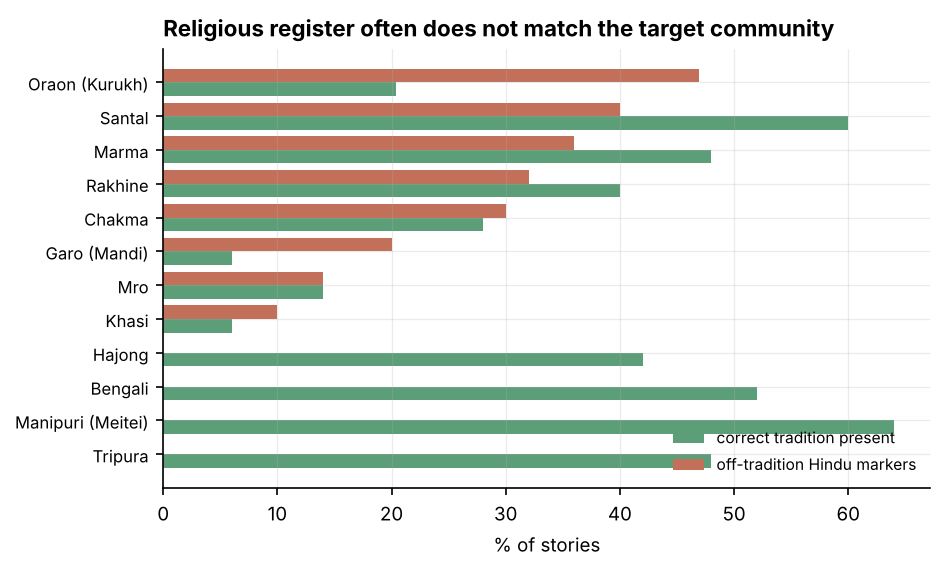
\includegraphics[width=\columnwidth]{figures/fig5_religious_leakage.png}
\caption{Religious register against target community. Hindu leakage is zero by
construction for the four communities where Hinduism is an expected tradition.}
\label{fig:religion}
\end{figure}

\paragraph{The scientific-intrusion hypothesis is false.}
A natural hypothesis is that models rationalise folk cosmology --- importing
``big bang'' framing into origin stories. They do not. Scientific register
appears in \textbf{2.7\%} of stories (cosmology 0.8\%, evolution and geology
0.3\%, matter and biology 0.3\%, science meta-vocabulary 1.2\%), and Origin
Stories show no elevation (3.4\% vs.\ 2.6\%, $p = 0.72$). Manual inspection of
every cosmology hit confirms they are poetic rather than rationalist: the
Manipuri origin story uses ``universe'' in ``the creator of the universe,
Tengbanba Mapu,'' which is correct Meitei cosmology. No story in the corpus
explains an origin scientifically.

This result must be read against the prompt, which explicitly prohibits modern
technology, modern statecraft, specific years and contemporary vocabulary. The
absence is therefore partly compliance, and it makes every modern term a
measurable instruction violation. Modern-world vocabulary still appears in
5.8\% of stories. The register that genuinely intrudes is contemporary
development and environmental ethics --- conservation, awareness, sustainability
--- in \textbf{11.9\%} of stories, concentrated sharply in gpt-5-mini (24.2\%)
and gemini (21.7\%) against gpt-5.1 (3.3\%) and mistral (2.5\%). It tracks the
explicit moral coda, and the best-rated model moralises least. The anachronism
in these stories is NGO register, not scientific register.

\paragraph{Instruction compliance inverts.}
Only 46.1\% of stories satisfy the 500--700 word instruction (gpt-5.1: 0.8\%,
99.2\% over; qwen: 1.7\%, 97.5\% under). Strikingly, stories that
\emph{violate} the length constraint are rated \emph{higher} (2.18 vs.\ 1.92,
$p = 2\times10^{-8}$), because the best model is the one that ignores it. The
benchmark's own length constraint is not what experts reward.

\subsection{Surface features predict nothing within a model}
\label{sec:confound}

Story length correlates with mean rating at $\rho = 0.36$ ($p < .001$) pooled,
the strongest single feature correlation we measured. It is entirely a
between-model artifact. Within each model the correlation vanishes: $-0.006$,
$-0.018$, $+0.058$, $-0.017$, $+0.176$, none significant at $.05$
(Figure~\ref{fig:length}). gpt-5.1 is both the longest and the best, but longer
gpt-5.1 stories are not better gpt-5.1 stories.

\begin{figure}[t]
\centering
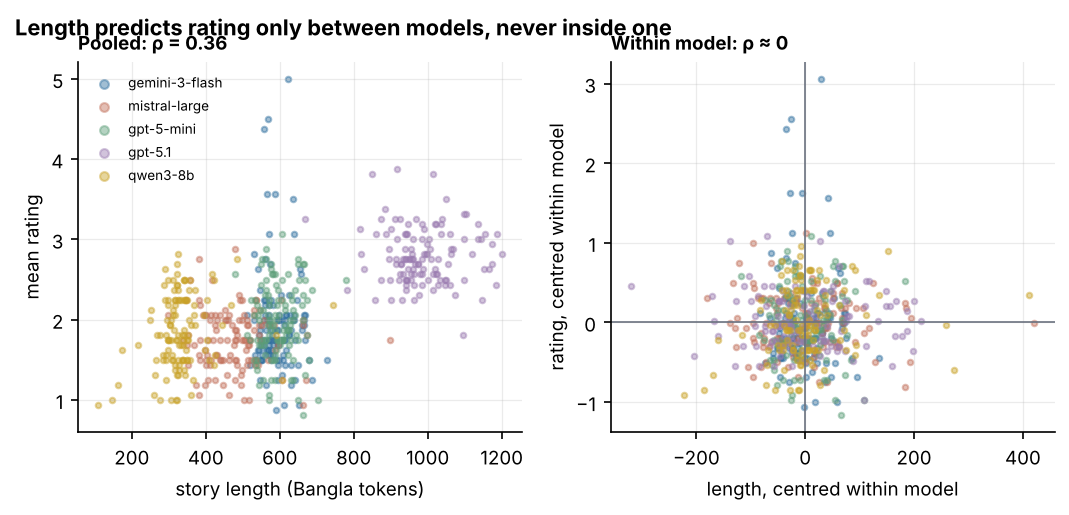
\includegraphics[width=\columnwidth]{figures/fig7_length_confound.png}
\caption{Length and rating, pooled and centred within model.}
\label{fig:length}
\end{figure}

This generalises. After group-mean-centring within model, of 19 features
$\times$ 4 dimensions the only robust survivors are Latin-script token count
predicting linguistic register ($\rho = 0.15$, $p < .001$) and narrative
coherence ($\rho = 0.11$, $p < .01$). Untransliterated indigenous terms are
rare --- 125 tokens corpus-wide, concentrated in Manipuri ritual vocabulary ---
but experts reward them. Otherwise no surface feature we computed predicts
expert judgment once model identity is held constant, which is a direct warning
against training automatic proxies on corpora of this shape.

\section{Discussion}
\label{sec:discussion}

The three results compose into one picture. Models possess real but shallow
cultural knowledge: correct community-specific terms exist in the corpus
(\S\ref{sec:flattening}) yet are deployed inconsistently, and the
religious life of some communities is omitted altogether
(\S\ref{sec:register}). What separates
good from bad output is not cultural difficulty but general capability
(\S\ref{sec:variance}). And the surface correlates of quality that a
cheap automatic metric would latch onto --- length, lexical diversity, cultural
word-marking --- are either between-model confounds or actively
anti-correlated with expert judgment (\S\ref{sec:flattening},
\S\ref{sec:confound}).

For \citet{pranida-etal-2025-culturally}, whose Javanese and Sundanese result
reports LLM--native parity on cultural fidelity, our reading is that parity is
fragile to the breadth of the culture axis: at twelve communities, with the
majority culture present as a control, fidelity does not hold.
\citet{chowdhury-etal-2025-facts} find that supplying context substantially
improves Bengali cultural knowledge, which suggests the most informative next
experiment is an ablation that supplies each model with a short, community-
specific cultural brief. If leakage collapses, the failure is retrieval; if it
persists, it is a genuine knowledge gap, and the two imply very different
remedies.

\section{Conclusion}

We release JAF, a fully crossed, fully expert-annotated corpus of 599
LLM-generated Bangla folk stories for twelve Bangladeshi communities. Expert
ratings show uniform failure with a ceiling of 2.79 of 5 and linguistic
register as the consistent floor. Pairing ratings with corpus analysis shows
that model identity dominates culture by a factor of 24 in explained variance,
that automatic culture-separability would invert the expert ranking, and that
the dominant failure mode is omission of expected cultural register rather
than scientific rationalisation. For eleven of the twelve communities studied, this
is to our knowledge the first evaluation of generative cultural competence of
any kind.

\section*{Limitations}

\paragraph{Scale and power.} Twelve cultures $\times$ five models $\times$ ten
story types with one generation per cell gives 599 items. This is adequate for
the model-level comparisons we report but underpowered for per-culture or
per-story-type claims, and we deliberately avoid them: the culture $R^2$ of
$0.017$ should be read as ``small relative to model,'' not as a precise
estimate. Single-sample generation also leaves decoding variance entirely
unmeasured; a re-run with multiple samples per cell could change the model
ordering, particularly for the four models clustered between 1.75 and 1.97.

\paragraph{Lexicon construction.} The religious, scientific, register and
development-ethics lexicons are hand-curated, and the leakage estimates are
only as good as their coverage. We mitigate this by separating strict from
generic religious markers, by whole-token rather than substring matching, and
by releasing the lexicons, but a term absent from a list is invisible to the
analysis. The Christian-marker result in particular rests on a short list, and
the correct reading is that the lexicon finds no Christian register in Garo and
Khasi stories, not that none could exist under a broader list.

\paragraph{Identifiability as a proxy.} Classifier accuracy measures lexical
distinguishability, not cultural correctness --- indeed demonstrating the gap
between them is one of our results. It should not be reused as a quality metric
elsewhere.

\paragraph{Annotator pool.} Four annotators rated all 599 items. Agreement is
high ($\alpha \ge 0.81$), but four raters cannot represent twelve distinct
communities, and we cannot establish from the released artifact whether any
annotator is a community insider for a given culture.
\authorfill{AUTHORS: this paragraph must be completed with the annotators' actual
relationship to the twelve communities. If no annotator is an insider for some
community, say so explicitly --- it is a material limitation for a cultural
authenticity judgment, and reviewers will ask.}

\paragraph{Corpus artifacts.} Every story in the corpus is a single paragraph;
no model produced paragraph breaks, whether through generation or
post-processing. Narrative structure above the sentence was therefore not
available to annotators, which likely depresses the coherence dimension in a
way that is an artifact of the pipeline rather than of the models.

\paragraph{Single prompt template.} One prompt template is used throughout.
The observed behaviours --- including the length violations and the moralising
coda --- may be specific to its phrasing, and prompt sensitivity is unmeasured.

\paragraph{Language scope.} All stories are in standard Bangla, including those
for communities with their own languages (Chakma, Khasi, Garo, Meitei, Kurukh).
This is deliberate, isolating cultural from multilingual competence, but it
means we evaluate how well models render a community \emph{in the majority
language}, which is a different and in some ways more fraught task than
generating in the community's own language.

\section*{Ethics Statement}

\paragraph{Representation of minority communities.} This work evaluates
machine-generated depictions of eleven minority communities in Bangladesh,
several of which have experienced documented marginalisation. The generated
stories are research artifacts and evaluation targets, not cultural
documentation, and must not be redistributed or presented as authentic
folklore of these communities. We report the omission of these communities' own religious register ---
complete, in the Garo and Khasi cases --- precisely because unexamined
deployment of such systems risks amplifying that erasure at scale.

\paragraph{Community consultation.}
\authorfill{AUTHORS: state whether any of the twelve communities were consulted in
designing the rubric or reviewing outputs, and if not, say so plainly. Also
state the IRB/ethics-board status of the annotation study (checklist D4) and
annotator compensation (D2).}

\paragraph{Release and licensing.} We release the corpus, annotations and
analysis code.
\authorfill{AUTHORS: specify the licence for the corpus and code, the terms under
which each model's outputs may be redistributed (provider terms differ), and
confirm that no personally identifying information appears in the generated
text (checklist B2--B4).}

\paragraph{Risk of misuse.} A corpus of synthetic folk narrative could be used
to generate plausible-looking but inauthentic cultural material at scale. Our
results indicate current models are poor at this task, which limits but does
not remove the risk.

\paragraph{Use of AI assistants.}
\authorfill{AUTHORS: checklist E1 requires a statement. Disclose any AI assistance
used in the analysis code, writing or corpus construction, per ACL policy.}

% Custom bibliography entries only
\bibliography{references,cultures}

\appendix

\clearpage
\section{The Twelve Communities}
\label{sec:cultures}

This appendix gives the background against which cultural accuracy was judged,
and documents the expected-tradition assignment used in \S\ref{sec:register}.
Population figures are from the 2022 Population and Housing Census
\cite{bbs2022census}, which enumerated 1{,}650{,}159 people in the official
ethnic-population category, roughly 1\% of the national population; Indigenous
organisations and researchers dispute the completeness of that count.
Community descriptions follow the relevant Banglapedia entries
\cite{banglapedia}, and language classifications follow Glottolog
\cite{glottolog}. No community is culturally uniform: denomination, village,
clan, generation, education and migration all produce internal variation, so
the descriptions below record historically documented patterns rather than
rules every present-day person follows.

\begin{table*}[t]
\centering\footnotesize
\setlength{\tabcolsep}{4pt}
\begin{tabular}{@{}p{2.0cm}p{3.5cm}p{3.3cm}p{4.4cm}r@{}}
\toprule
Community & Principal region & Language (family) & Predominant tradition & 2022 census \\
\midrule
Bengali           & Nationwide                      & Bangla (Indo-Aryan)         & Muslim majority, Hindu minority & --- \\
Chakma            & Rangamati, Khagrachhari         & Chakma (Indo-Aryan)         & Theravada Buddhist              & 483{,}299 \\
Marma             & Bandarban, Rangamati            & Marma (Sino-Tibetan)        & Theravada Buddhist              & 224{,}261 \\
Tripura           & Khagrachhari                    & Kokborok (Sino-Tibetan)     & Indigenous and Hindu            & 156{,}578 \\
Santal            & Rajshahi, Rangpur plains        & Santali (Austroasiatic)     & Indigenous \textit{bonga}; Christian minority & 129{,}049 \\
Oraon (Kurukh)    & Rajshahi, Rangpur; tea estates  & Kurukh (Dravidian)          & Indigenous \textit{Dharmes}; Christian, some Hindu & 85{,}846 \\
Garo (Mandi)      & Mymensingh, Sherpur             & Mandi/A'chik (Sino-Tibetan) & \textbf{Christian majority} (Catholic, Baptist) & 76{,}846 \\
Mro               & Bandarban                       & Mro (Sino-Tibetan)          & Indigenous; some Buddhist       & 52{,}455 \\
Manipuri (Meitei) & Moulvibazar, Sylhet             & Meitei (Sino-Tibetan)       & Gaudiya Vaishnava Hindu         & 22{,}978 \\
Khasi             & Sylhet border hills             & Khasi (Austroasiatic)       & \textbf{Christian majority} ($>$80\%, Presbyterian) & 12{,}421 \\
Rakhine           & Cox's Bazar, Patuakhali         & Rakhine (Sino-Tibetan)      & Theravada Buddhist              & 11{,}195 \\
Hajong            & Netrokona, Sherpur              & Hajong (Indo-Aryan)         & Hindu (Shakta, Vaishnava)       & 7{,}996 \\
\bottomrule
\end{tabular}
\caption{The twelve communities. Religious tradition determines the
expected-tradition mapping in \S\ref{sec:register}; the two Christian-majority
communities are highlighted. Chakma, Marma, Mro and Tripura are Chittagong
Hill Tracts communities. Census counts from \citet{bbs2022census};
descriptions from \citet{banglapedia}; families from \citet{glottolog}.}
\label{tab:cultures}
\end{table*}

\paragraph{Why the religious mapping matters.} Table~\ref{tab:cultures} is the
ground truth behind \S\ref{sec:register}. Banglapedia records that over 80\% of
Bangladeshi Khasi are Christian, mostly Protestant
\cite{banglapedia-khasia}, and that most Garo are now Christian, divided
between a Roman Catholic majority and Baptist and other Protestant churches
\cite{banglapedia-garo}. These are the two communities for which the corpus
contains no Christian marker at all. For the Theravada Buddhist communities
(Chakma, Marma, Rakhine) the expected register includes the monastery
(\bn{কিয়াং} \textit{kyang}) and the monk (\bn{ভান্তে} \textit{bhante}); for
Santal and Oraon it includes the sacred grove and indigenous deities rather
than a temple.

\paragraph{Three cultural-geographic zones.} The communities fall into zones
that explain the confusion structure reported in \S\ref{sec:flattening}. The
\emph{Chittagong Hill Tracts} hold Chakma, Marma, Mro and most Tripura, who
share swidden cultivation (\bn{জুম} \textit{jum}), hill-stream ecology and, for
three of the four, Theravada Buddhism --- which is why the classifier confuses
them with one another. The \emph{northwestern plains} hold Santal and Oraon,
whose shared agrarian ritual calendar and sal-forest ecology likewise produce
mutual confusion. The \emph{northeastern and coastal margins} hold Khasi,
Manipuri, Garo and Hajong near the Indian border and Rakhine along the
southern coast.

\paragraph{Language and the Bangla-output design.} Only Chakma, Hajong and
Bengali are Indo-Aryan. Kurukh is Dravidian --- the only Dravidian language in
Bangladesh. Santali and Khasi are Austroasiatic, and the remainder are
Sino-Tibetan \cite{glottolog}. Requiring all output in standard Bangla
therefore asks the model to render, in a majority Indo-Aryan language, the
cultural world of communities speaking languages from four unrelated families.
This isolates cultural from multilingual competence, as intended, but it is
also the condition under which the glossing behaviour discussed in
\S\ref{sec:register} arises: a model writing about a Santal \bn{নায়কে}
\textit{naeke} in Bangla has no religiously neutral Bangla word for the role.

\paragraph{Selected community notes.} \textbf{Chakma} are the largest
enumerated Indigenous community; their language is Indo-Aryan despite their
location among Sino-Tibetan-speaking neighbours, and they have their own
script. \textbf{Garo} and \textbf{Khasi} are both matrilineal: Garo children
take the mother's surname with the youngest daughter typically inheriting, and
Khasi descent and property likewise pass through women, with the village
(\bn{পুঞ্জি} \textit{punji}) and clan as core units; Khasi livelihood is
strongly associated with betel-leaf cultivation. \textbf{Santal} religious life
centres on the sacred grove (\bn{জাহের} \textit{jaher}) and \textit{Marang
Buru}. \textbf{Oraon} inherited religion centres on \textit{Dharmes},
associated with the sun, with the \textit{Karam} festival and the \textit{pahan}
priest as salient institutions. \textbf{Manipuri} follow Gaudiya Vaishnavism,
so temple and \textit{mandap} vocabulary is appropriate for them and not for
most others --- the one community where Hindu register is expected rather than
anomalous. \textbf{Rakhine} settled the southern coast from Arakan in the late
eighteenth century, and maritime life figures centrally in their narrative
repertoire.

\paragraph{Terminology.} The terminology for these communities is politically
contested in Bangladesh. The Constitution refers to ``tribes, minor races,
ethnic sects and communities,'' while many community organisations prefer
``Indigenous Peoples'' or \textit{Adivasi}, a difference bound up with debates
over self-identification, customary institutions and land rights. We use each
community's own name where possible and otherwise ``community,'' without
implying that every individual adopts the same political terminology.

\section{Reproducibility}
\label{sec:appendix}

\paragraph{Text processing.} All textual measures operate on Bangla-script word
tokens matched whole, with a light inflectional suffix matcher; substring
matching inflates counts by an order of magnitude on common terms
(\S\ref{sec:beyond}). The tokeniser, stopword list and lexicons are released
with the analysis code, along with unit tests pinning the matching behaviour.

\paragraph{Agreement estimators.} Krippendorff's $\alpha$ uses the ordinal
difference metric. We validate the implementation on synthetic boundary cases
--- perfect agreement, random coding, signal-plus-noise and restricted-range
conditions --- and release those as tests, because an incorrectly normalised
implementation can return plausible-looking values on real data while failing
on random input.

\paragraph{Statistical procedures.} Group comparisons use Mann--Whitney $U$ with
Cohen's $d$ reported for effect size. Classifier results are five-fold
stratified cross-validation with TF-IDF features and logistic regression.
Distinctive vocabulary uses the log-odds ratio with an informative Dirichlet
prior, with the corpus itself as prior. Within-model analyses use group-mean
centring on both the feature and the rating.

\paragraph{Typesetting.} Bangla examples are set in Kalpurush via
\texttt{fontspec} with \texttt{Script=Bengali}; the paper must be compiled with
XeLaTeX, since pdf\LaTeX{} cannot perform the conjunct substitutions and
renders ligatures such as \bn{ব্রাহ্মণ} as broken glyph sequences. Word clouds
in the released analysis have the same requirement. Chart labels are in English
because the plotting library does not shape Bangla.

\end{document}
